%%% Sekce - Dokončení objednávky
%%%%% Wording: ✅
%%%%% Styling: ✅
%%%%% References: ✅
%%%%% Grammar: ✅
%%% --------------------------------------------------------------
\section{Dokončení objednávky}
\label{sec:identifikace-dokonceni-objednavky}
Jakmile si zákazník vybere požadované vstupenky a rezervovaná místa, je jeho posledním úkolem dokončit a tím tak vytvořit objednávku, kterou následně zaplatí.
Tento proces je většinou rozdělen do několika kroků, které zákazníka postupně provedou celým procesem dokončení objednávky.

Tato podkapitola se bude těmito kroky zabývat a bude se snažit popsat jejich jednotlivé části a funkčnosti, které by měly být v takovémto systému implementovány.

Avšak je nutné nejprve uvést, že následující funkčnosti jsou v práci uvedené pouze z důvodu kompletnosti představení celého procesu nákupu vstupenek s rezervací míst a záměrně nebudou v rámci praktické části plně implementovány nýbrž pouze orientačně využity – a to z důvodu toho, že se jedná, již převážně o funkčnosti a procesy na straně backendového systému a ne frontendového, který je předmětem této práce.

%%% Podsekce - Osobní informace
%%%%% Wording: ✅
%%%%% Styling: ✅
%%%%% References: ✅
%%%%% Grammar: ✅
%%% --------------------------------------------------------------
\begin{subsection}{Osobní informace}
    \label{subsec:identifikace-dokonceni-objednavky-osobni-informace}
    Pro účely dokončení objednávky je nutné, aby si zákazník vyplnil své osobní informace, které jsou potřebné pro vytvoření objednávky a následné doručení vstupenek.
    Tyto informace by měly obsahovat minimálně následující údaje:

    \begin{itemize}
        \item Jméno a příjmení
        \item Emailová adresa
        \item Telefonní číslo
    \end{itemize}

    Tyto informace jsou nezbytné například pro odeslání potvrzení objednávky, doručení vstupenek či poskytování případné podpory zákazníkům.

    Někteří poskytovatelé stále nabízí doručení fyzických vstupenek na adresu zákazníka, nicméně tento způsob je spíše přežitek.
    V dnešní moderní době je výhodnější i ekologičtější využít možnost digitálních vstupenek, které zákazník obdrží v elektronické podobě například prostřednictvím emailu či SMS zprávy.

    V rámci dokončení objednávky je také časté vybídnutí zákazníka k dokončení registrace na dané platformě či službě, přes kterou vstupenky nakupuje.
    Tato registrace je většinou dobrovolná, ale může být i povinná, pokud chce zákazník využít některé z výhod, které jsou s touto registrací spojeny.
\end{subsection}

%%% Podsekce - Výběr platební metody
%%%%% Wording: ✅
%%%%% Styling: ✅
%%%%% References: ✅
%%%%% Grammar: ✅
%%% --------------------------------------------------------------
\begin{subsection}{Výběr platební metody}
    \label{subsec:identifikace-dokonceni-objednavky-vyber-platebni-metody}
    Proces dokončení objednávky by v posledním kroku měl zákazníkovi nabídnout několik možností platby.
    Tato část velmi úzce souvisí s implementací backendového systému, který není součástí této práce, a proto tato sekce bude pouze orientační a bude se snažit popsat možnosti, které by měly být v takovémto systému implementovány.
    Nejčastějšími platebními metodami jsou:

    \begin{itemize}
        \item platba kartou
        \item platba přes PayPal
        \item platba přes Apple Pay
        \item platba přes Google Pay
        \item platba přes bankovní převod
    \end{itemize}

    \begin{figure}[H]
        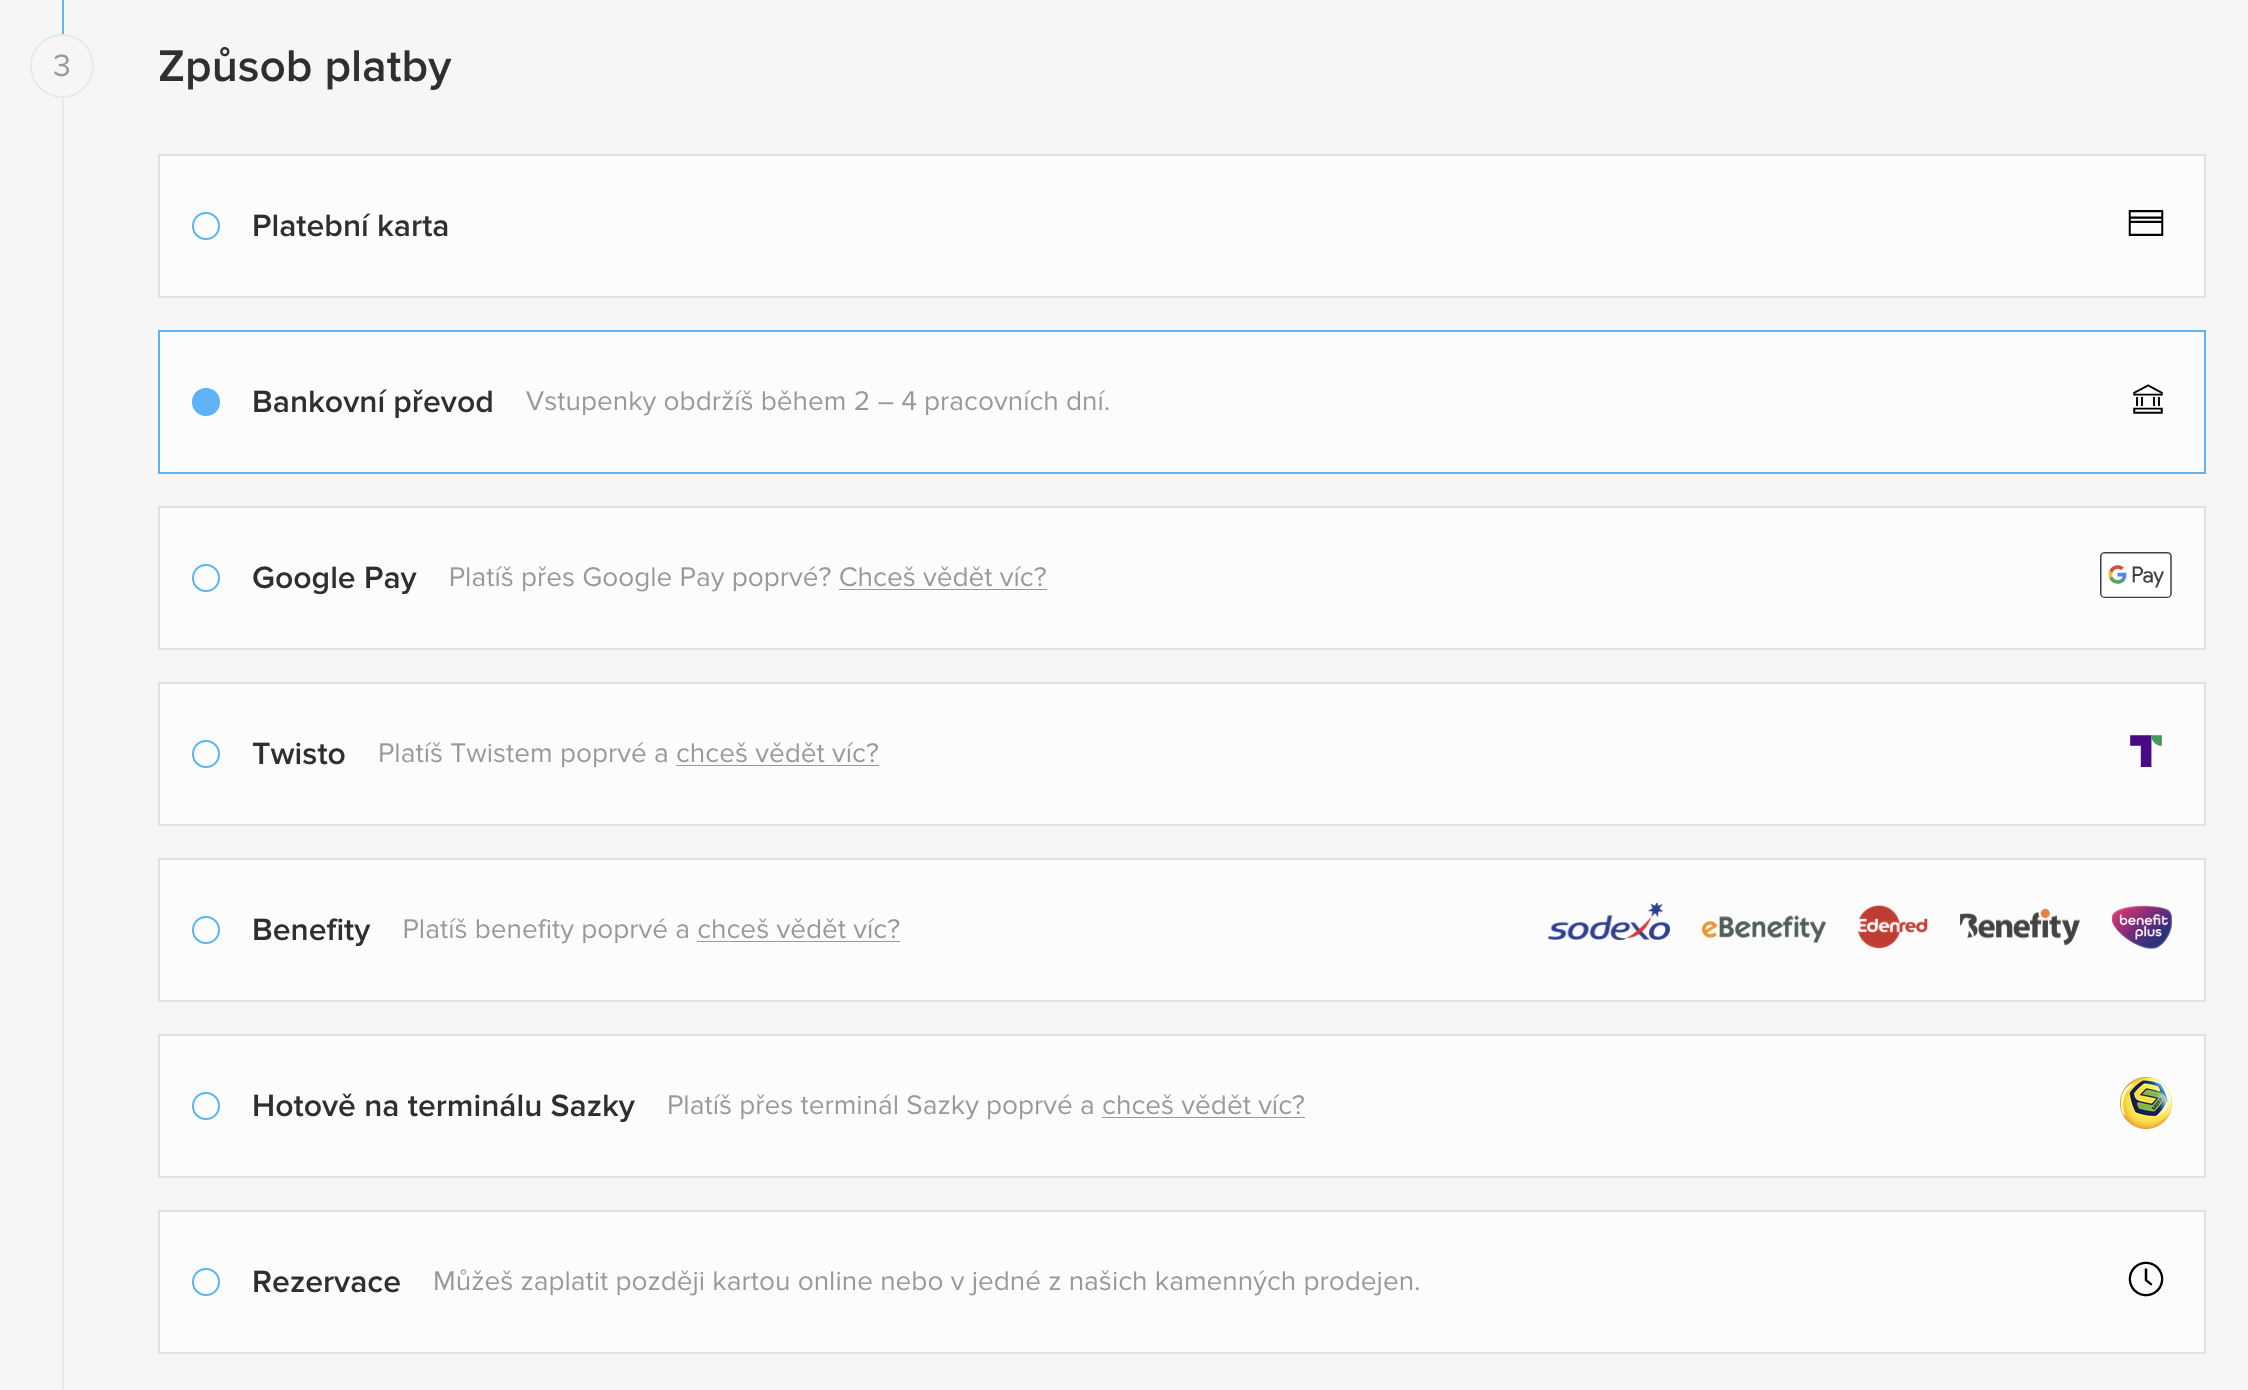
\includegraphics[width=\linewidth]{\FIGDIR/goout-payment-methods}
        \centering
        \caption{Výběr platební metody na GoOut.net\cite{g__goout_net}}
        \label{fig:goout-payment-methods}
    \end{figure}

    Na obrázku~\ref{fig:goout-payment-methods} je vidět výběr platební metody ve službě GoOut.net, která nabízí výše zmíněné platební metody\footnote{platební metoda Apple Pay zde není uvedena, jelikož je dostupná pouze v rámci prohlížečů Safari: \url{https://support.apple.com/guide/iphone/use-apple-pay-in-apps-app-clips-and-safari-iph67e89f7c8/ios}} spolu i dalšími jako například platba přes službu Twisto\footnote{Twisto je služba, která umožňuje zákazníkům platit za zboží a služby až po jejich doručení. Zákazník tak může využít služeb Twisto až do 45 dní bez úroků a poplatků.\url{https://www.twisto.cz/}} či Sodexo\footnote{Sodexo je společnost, která poskytuje zaměstnanecké benefity jako například stravenky, dárkové poukazy, karty a mobilní aplikace. \url{https://www.sodexo.cz/}} a další jiné benefitní programy.

    Pro účely platby kartou je nutné, aby byl zákazník přesměrován na platební bránu, která je schopna tuto platbu zpracovat.
    Většinou se jedná o platební brány třetích stran, které jsou schopny zpracovat platby z různých platebních karet a poskytovatelů.
    Mezi nejznámější poskytovatele platebních brán na českém trhu patří například:

    \begin{itemize}
        \item \textbf{Comgate} (\url{https://www.comgate.cz/platebni-brana})
        \item \textbf{GoPay} (\url{https://www.gopay.com/cs/})
        \item \textbf{PayU} (\url{https://czech.payu.com/payu-moderni-platebni-reseni/})
        \item \textbf{GP webpay} (\url{https://www.gpwebpay.cz/})
        \item \textbf{Stripe} (\url{https://stripe.com/en-cz})
    \end{itemize}

    Na obrázcích~\ref{fig:comgate-fees-table} a~\ref{fig:comgate-payment-methods} je vidět, že každý poskytovatel platební brány nabízí jiné výhody a poplatkové modely, nicméně všechny mají společné to, že zpracovávají platby z různých platebních karet a poskytovatelů a přímo podporují i mobilní platby přes Apple Pay a Google Pay.

    \begin{figure}[H]
        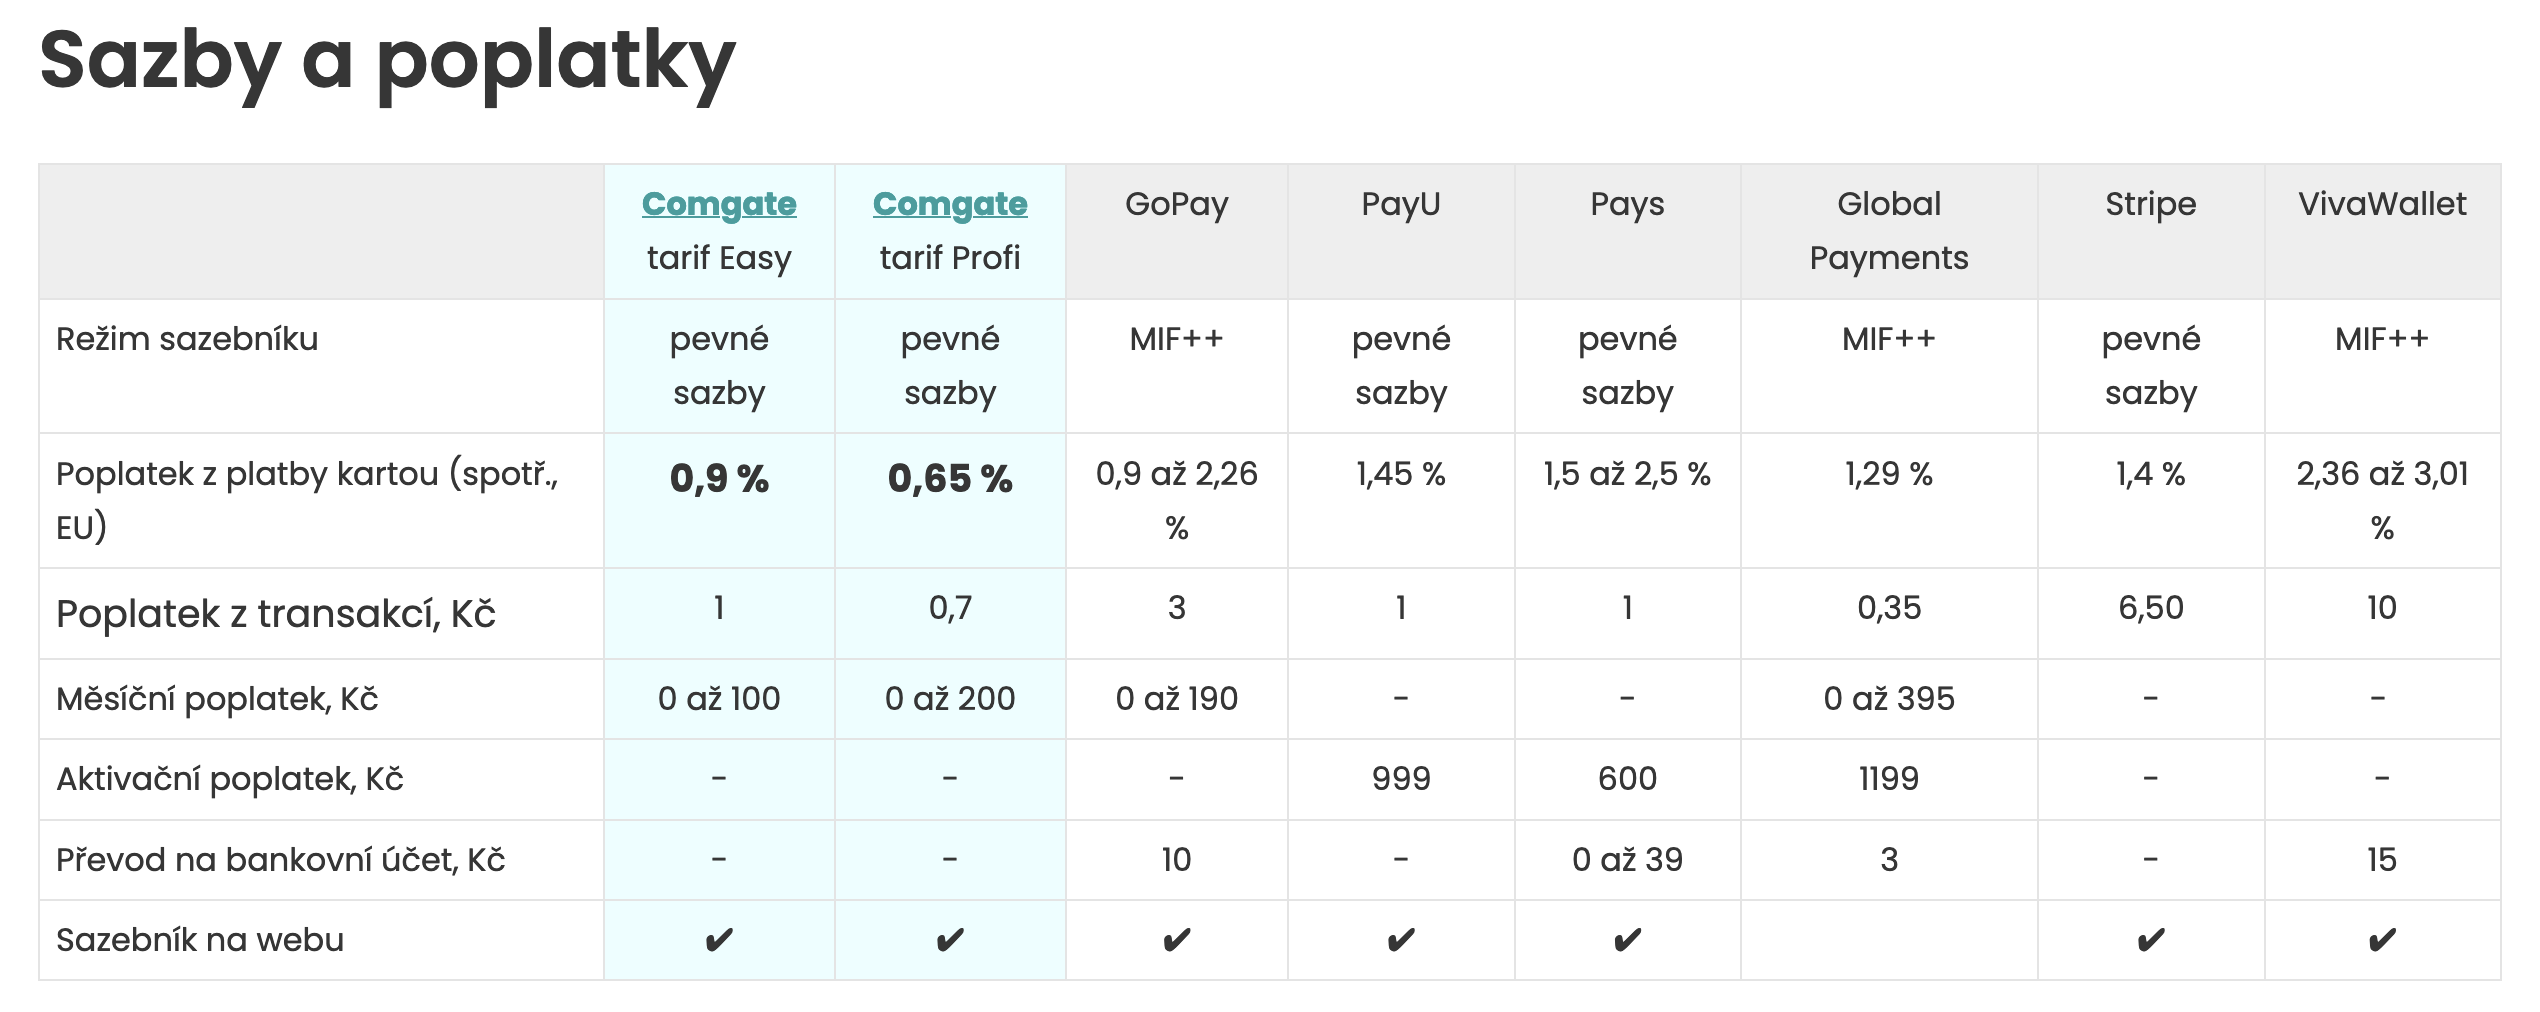
\includegraphics[width=\linewidth]{\FIGDIR/comgate-fees-table}
        \centering
        \caption{Srovnání platebních bran dle Comgate.cz~\cite{comgate_srovnani_platebnich_bran}}
        \label{fig:comgate-fees-table}
    \end{figure}

    \begin{figure}[H]
        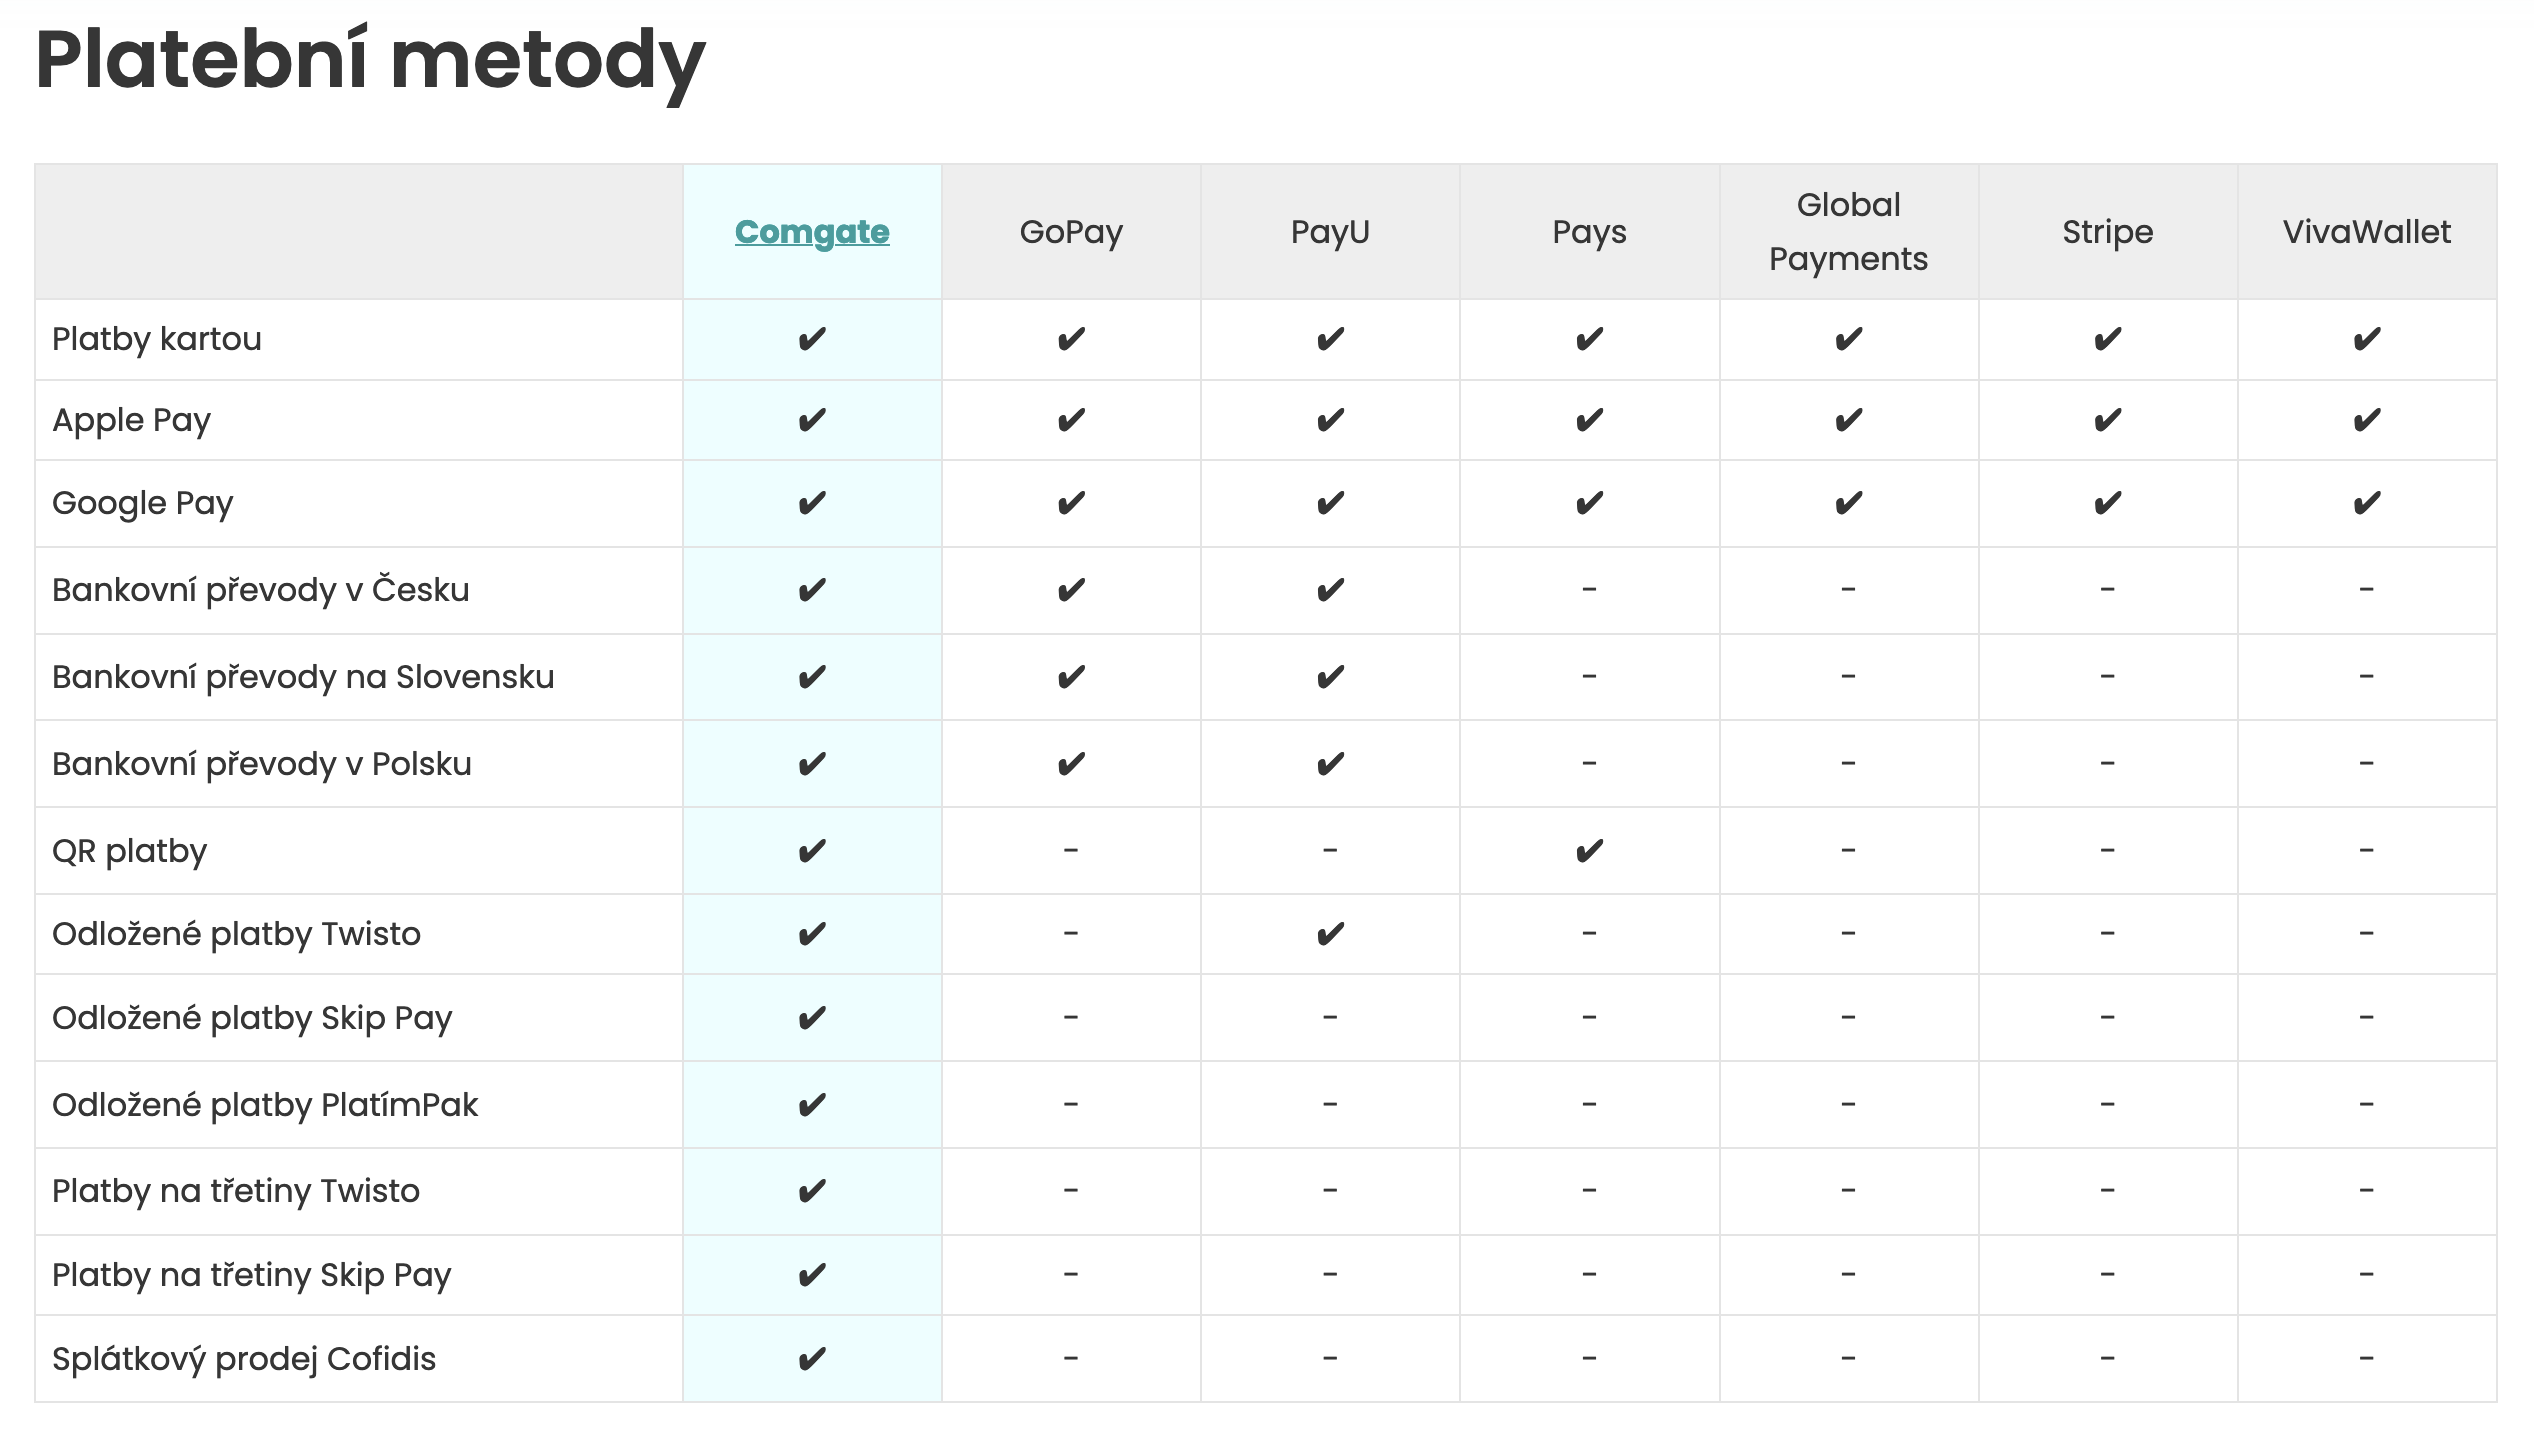
\includegraphics[width=\linewidth]{\FIGDIR/comgate-payment-methods}
        \centering
        \caption{Platební metody poskytované platebními poskytovateli dle Comgate.cz~\cite{comgate_srovnani_platebnich_bran}}
        \label{fig:comgate-payment-methods}
    \end{figure}

    Některé e-shopy však nabízí i vlastní platební bránu, nicméně tato možnost je spíše výjimkou.
    Stát se provozovatelem vlastní platební brány je totiž velmi náročné na vývoj, údržbu a provoz a je k němu nutné mít i licenci platební instituce (PI)\cite{schejbal_platebni_instituce}, kterou vydává Česká národní banka (ČNB)\cite{cnb_dohled_platebni_instituce}.

    Platby přes bankovní převod mohou být pro poskytovatele řešení prodeje vstupenek velmi výhodné, jelikož se jedná o levnější způsob převodu peněz, než je tomu u plateb kartou.
    Platební brány si totiž účtují poplatky za zpracování každé z plateb, a to nejčastěji v režimu pevného sazebníku či MIF++ modelu\footnote{někdy také označován jako Interchange++}, který rozděluje poplatky mezi vydavatelskou bankou, karetním schématem (např.\ Visa, MasterCard) a platební bránou\cite{gp_podpora_mif}.

    Do nedávna mohla být platba bankovním převodem pro zákazníky stále méně oblíbená, jelikož bylo nutné počkat na připsání peněz na účet poskytovatele, což mohlo trvat i několik dní.
    V dnešní době je však možné využít tzv.
    instantní platby, které jsou schopny převést peníze mezi účty různých bank během několika sekund.
    V České republice aktuálně podporuje instantní platby již několik bank, jako například Komerční banka, a.s., MONETA Money Bank, a.s.\ či Fio banka, a.s.\ a další\footnote{kompletní seznam účastníků okamžitých plateb dle ČNB dostupný z: \url{https://www.cnb.cz/export/sites/cnb/cs/platebni-styk/.galleries/certis/download/seznam_okamzite_platby.pdf}}.
\end{subsection}

%%% Podsekce - Souhrn objednávky
%%%%% Wording: ✅
%%%%% Styling: ✅
%%%%% References: ✅
%%%%% Grammar: ✅
%%% --------------------------------------------------------------
\begin{subsection}{Souhrn objednávky}
    \label{subsec:identifikace-dokonceni-objednavky-souhrn-objednavky}
    Po vyplnění všech potřebných informací a výběru platební metody by zákazníkovi měl být před finálním potvrzením objednávky zobrazen její souhrn.
    Tento souhrn zákazníkovi umožní zkontrolovat, zda jsou všechny údaje správně vyplněné a zda je vše v pořádku.
    Pokud zákazník zjistí, že je něco špatně, měl by mít možnost vrátit se zpět a údaje opravit.
    Pokud je vše v pořádku, měl by mít možnost objednávku potvrdit a přejít k platebnímu procesu.

    Součástí potvrzení objednávky také často bývá zaškrtnutí souhlasu se zpracováním osobních údajů a obchodních podmínek či i případně dalších informací, jako například zasílání novinek a reklamních nabídek na e-mailovou adresu zákazníka.
\end{subsection}

%%% Podsekce - Vytvoření objednávky a potvrzení
%%%%% Wording: ✅
%%%%% Styling: ✅
%%%%% References: ✅
%%%%% Grammar: ✅
%%% --------------------------------------------------------------
\begin{subsection}{Vytvoření objednávky a potvrzení}
    \label{subsec:identifikace-dokonceni-objednavky-vytvoreni-objednavky-a-potvrzeni}
    Po potvrzení objednávky by měla být vytvořena objednávka v databázi a zákazníkovi by mělo být zobrazeno potvrzení o jejím vytvoření.
    Na základě vybrané platební metody by měl být dále přesměrován k jejímu zaplacení a posléze zpět na detail objednávky s potvrzením o zaplacení.
    Při úspěšné platbě by zákazníkovi měl systém doručit zakoupené vstupenky v elektronické podobě, například v podobě PDF souboru, který bude obsahovat vstupenky ve formátu QR kódu.
    Tato funkčnost je opět úzce spjata s backendovým systémem, který ale aktuální rozsah práce nepokrývá.
\end{subsection}
